
\begin{frame}{SALAMANDER}
  \begin{columns}
    \column{0.6\textwidth}
    \vspace{1.1cm}
    \begin{itemize}
      \item SALAMANDER \textemdash{} Software for Advanced Large-scale Analysis of Magnetic confinement for Numerical Design, Engineering \& Research.\cite{salamander2025}
      \begin{itemize}
          \item Open Source.
      \end{itemize}
      \begin{itemize}
        \item Built upon MOOSE \textemdash{} a massively parallel finite-element method (FEM) framework.
      \end{itemize}
       \item FEM particle-in-cell (PIC) capabilities are being developed within SALAMANDER.
      \begin{itemize}
        \item Built on MOOSE's Ray Tracing module.
        \begin{itemize}
            \item Scalable with $\sim$18,500 MPI ranks.\cite{gaston2021method}
        \end{itemize}
        \item Supports structured and unstructured meshes in 1D, 2D, and 3D.
      \end{itemize}
    \end{itemize}
    \column{0.5\textwidth}
    \centering
    Multiphysics Divertor Monoblock Model
    \vspace{-0.6cm}
    \begin{figure}
    \begin{tikzpicture}
      \node[anchor=south west, inner sep=0] (image1) at (0,0) {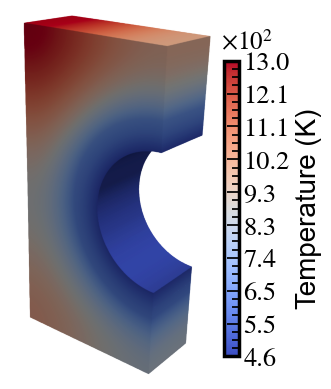
\includegraphics[height=0.5\textheight]{figs/temperature_output.png}};
      \node[anchor=north west, inner sep=0] (image2) at ([xshift=-0.3cm,yshift=0cm]image1.north east)
      {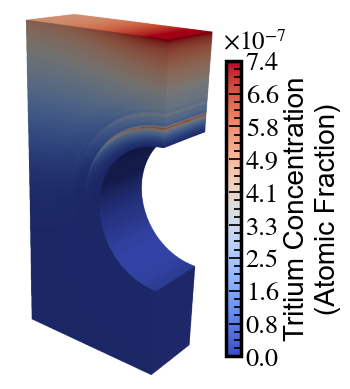
\includegraphics[height=0.5\textheight]{figs/tritium_output.png}};
    \end{tikzpicture}
    \end{figure}
    \vspace{-1.5cm}
  \end{columns}
\end{frame}

\begin{frame}{Software Quality and Motivation}
  \vspace{0.5cm}
  \begin{columns}
    \column{0.5\textwidth}
    \begin{itemize}
        \item SALAMANDER is being developed with nuclear quality software quality assurance practices.
        \item Rigorous verification and testing are a core part of the development process.
        \item At low pressures, neutral particles are also kinetic, requiring direct simulation Monte Carlo (DSMC)\cite{bird1994molecular}.
        \item In this work, two kinetic problems demonstrate the initial implementation of the DSMC algorithm.
    \end{itemize}
    \column{0.5\textwidth}
    \begin{figure}
    \begin{tikzpicture}
      \node[anchor=south west, inner sep=0] (image2) at (3.1,-2.25) {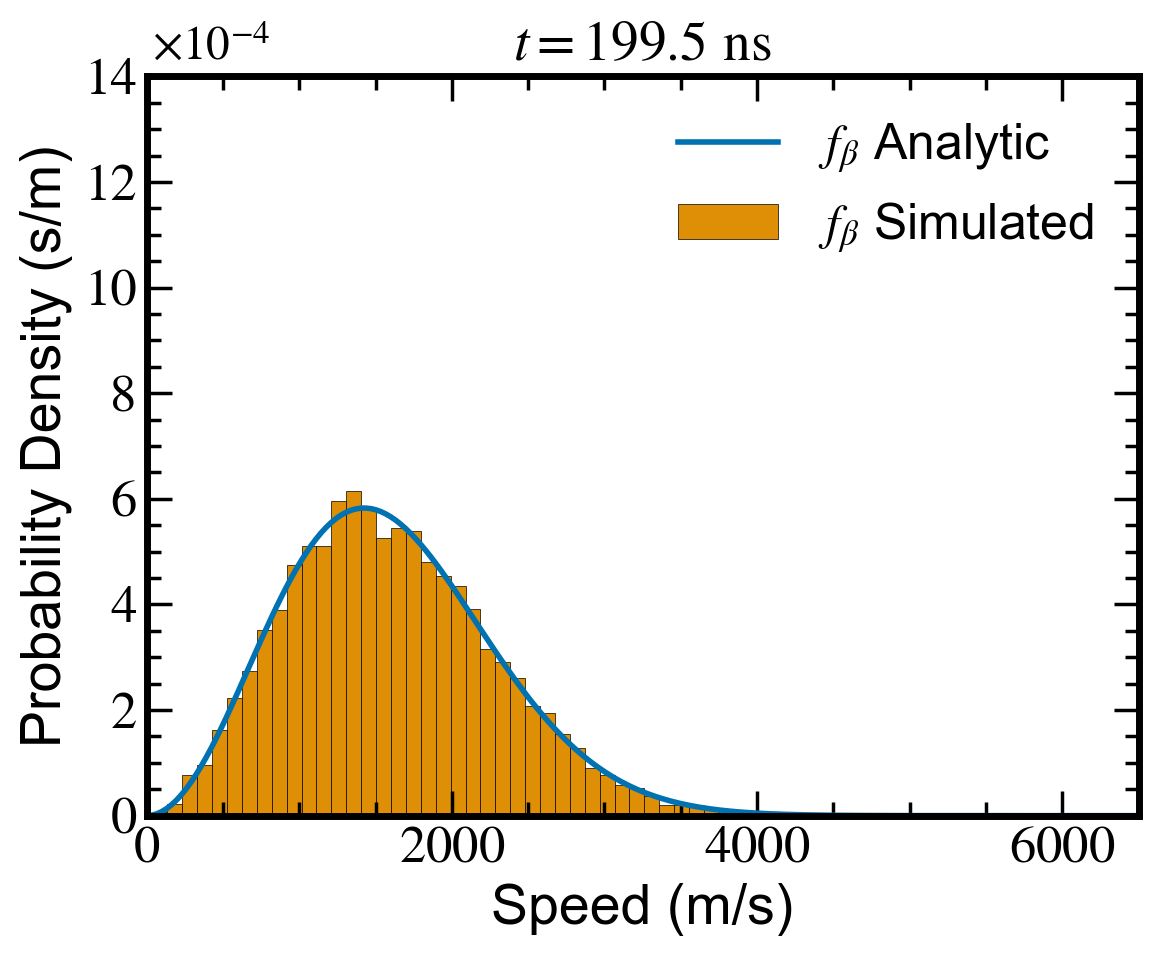
\includegraphics[width=0.65\textwidth]{gifs/beta_frames/frame.199.png}};
      \filldraw[white] (3.19, 0.58) rectangle (4.475, 1.8);
      \filldraw[white] (3.19, 0.45) rectangle (3.45, 0.6);
      \node[anchor=south west, inner sep=0] (image1) at (0,0) {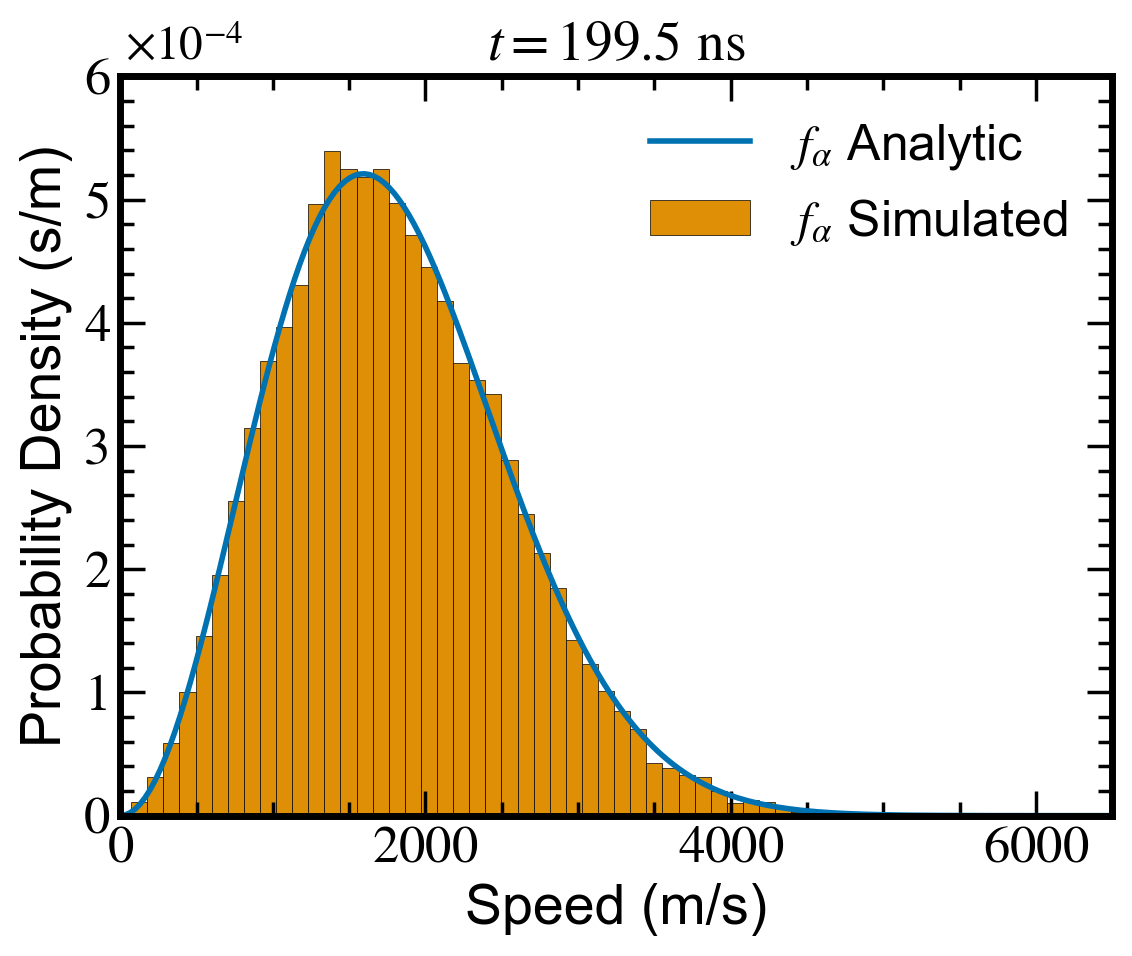
\includegraphics[width=0.65\textwidth]{gifs/alpha_frames/frame.199.png}};
    \end{tikzpicture}
    \end{figure}
  \end{columns}
\end{frame}

\begin{frame}{PIC Design and Simulation Flow}
  \begin{columns}
  \column{0.5\textwidth}
  \vspace{1cm}
  \begin{itemize}
    \item Particles shape functions are Dirac delta functions.
    \item Particles are pushed with the leap frog or Boris method.
    \item In an element, particle weight, $w$, is based on number density $n$, element volume $V_E$, and particles per element $N_p$.
    \begin{align*}
        w = \frac{n V_E}{N_p}
    \end{align*}
    \item The DSMC method is used for collisions.
  \end{itemize}
  \column{0.5\textwidth}
    \begin{figure}[H]
    \resizebox{\columnwidth}{!}{
      \begin{tikzpicture}[
        auto,
        node distance = 1cm,
        very thick,
        algoBlue/.style={rectangle,
        draw=NCSURed,
        font=\bfseries\boldmath,
        text width=3.5cm,
        align=center,
        rounded corners=2.5mm},
        auto,
        line width = 2pt
        ]
        \node[algoBlue] (1) [yshift=0.25cm] {Initialize particles};
        \node[algoBlue] (2) [yshift=-1.25cm] {Calculate $\vec{v}_{n+1/2}$ using $\vec{E}_n$ and $\vec{B}_n$};
        \draw[line width=0.3mm, >=triangle 45, ->] (1) -- (2);
        %
        \node[algoBlue] (3) [xshift=2.3cm, yshift=-2.75cm] {Move particles to $\vec{r}_{n+1}$ using $\vec{v}_{n+1/2}$};
        \draw[line width=0.3mm, >=triangle 45, ->] (2.east) -| (3.north);
        \node[algoBlue] (5) [xshift=2.3cm, yshift=-4.5cm] {Compute $\left< \rho_{n+1}, \psi \right>$ based on $\vec{r}_{n+1}$};
        \draw[line width=0.3mm, >=triangle 45, ->] (3.south) -- (5.north);
        \node[algoBlue] (6)  [xshift=-2.3cm, yshift=-4.5cm]
        {Compute ${\phi}_{n+1}$ and $\vec{E}_{n+1}$};
        \draw[line width=0.3mm, >=triangle 45, ->] (5.west) -- (6.east);
        \node[algoBlue] (7)  [xshift=-2.3cm, yshift=-2.75cm]
        {Particle\\collisions};
        \draw[line width=0.3mm, >=triangle 45, ->] (6) -- (7);
        \draw[line width=0.3mm, >=triangle 45, ->] (7.north) |- (2.west);
      \end{tikzpicture}
      }
    \end{figure}
\end{columns}
\end{frame}

\begin{frame}{Previous Verification}
  \begin{columns}
    \column{0.45\textwidth}
    \begin{itemize}
      \item Fundamental PIC capabilities have been verified.\cite{gall2024kinetic}
      \begin{itemize}
        % \item Single partille motion.
        \item Electrostatic potential solve.
        \item Density projection onto the mesh.
        \item Charge conservative current density calculations.
        \item Two stream and Dory-Guest-Harris instabilities.
      \end{itemize}
      \item Previous verification is/will be available:
      \customlink{https://github.com/idaholab/salamander}
    \end{itemize}
    \column{0.55\textwidth}
    % \begin{figure}[H]
    %   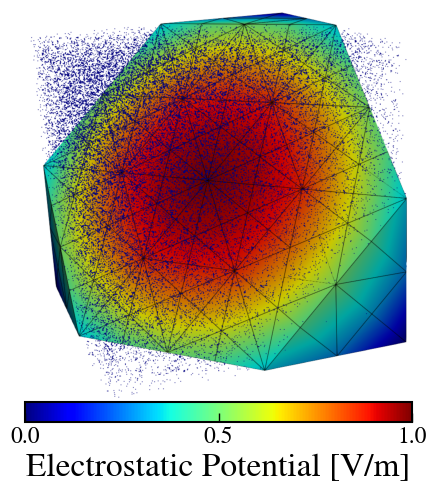
\includegraphics[width=0.9\textwidth]{figs/potential_visualiation.png}
    %  \end{figure}
    \begin{figure}
    \begin{tikzpicture}
  % First image at (0,0)
      \node[anchor=south west, inner sep=0] (image1) at (0,0) {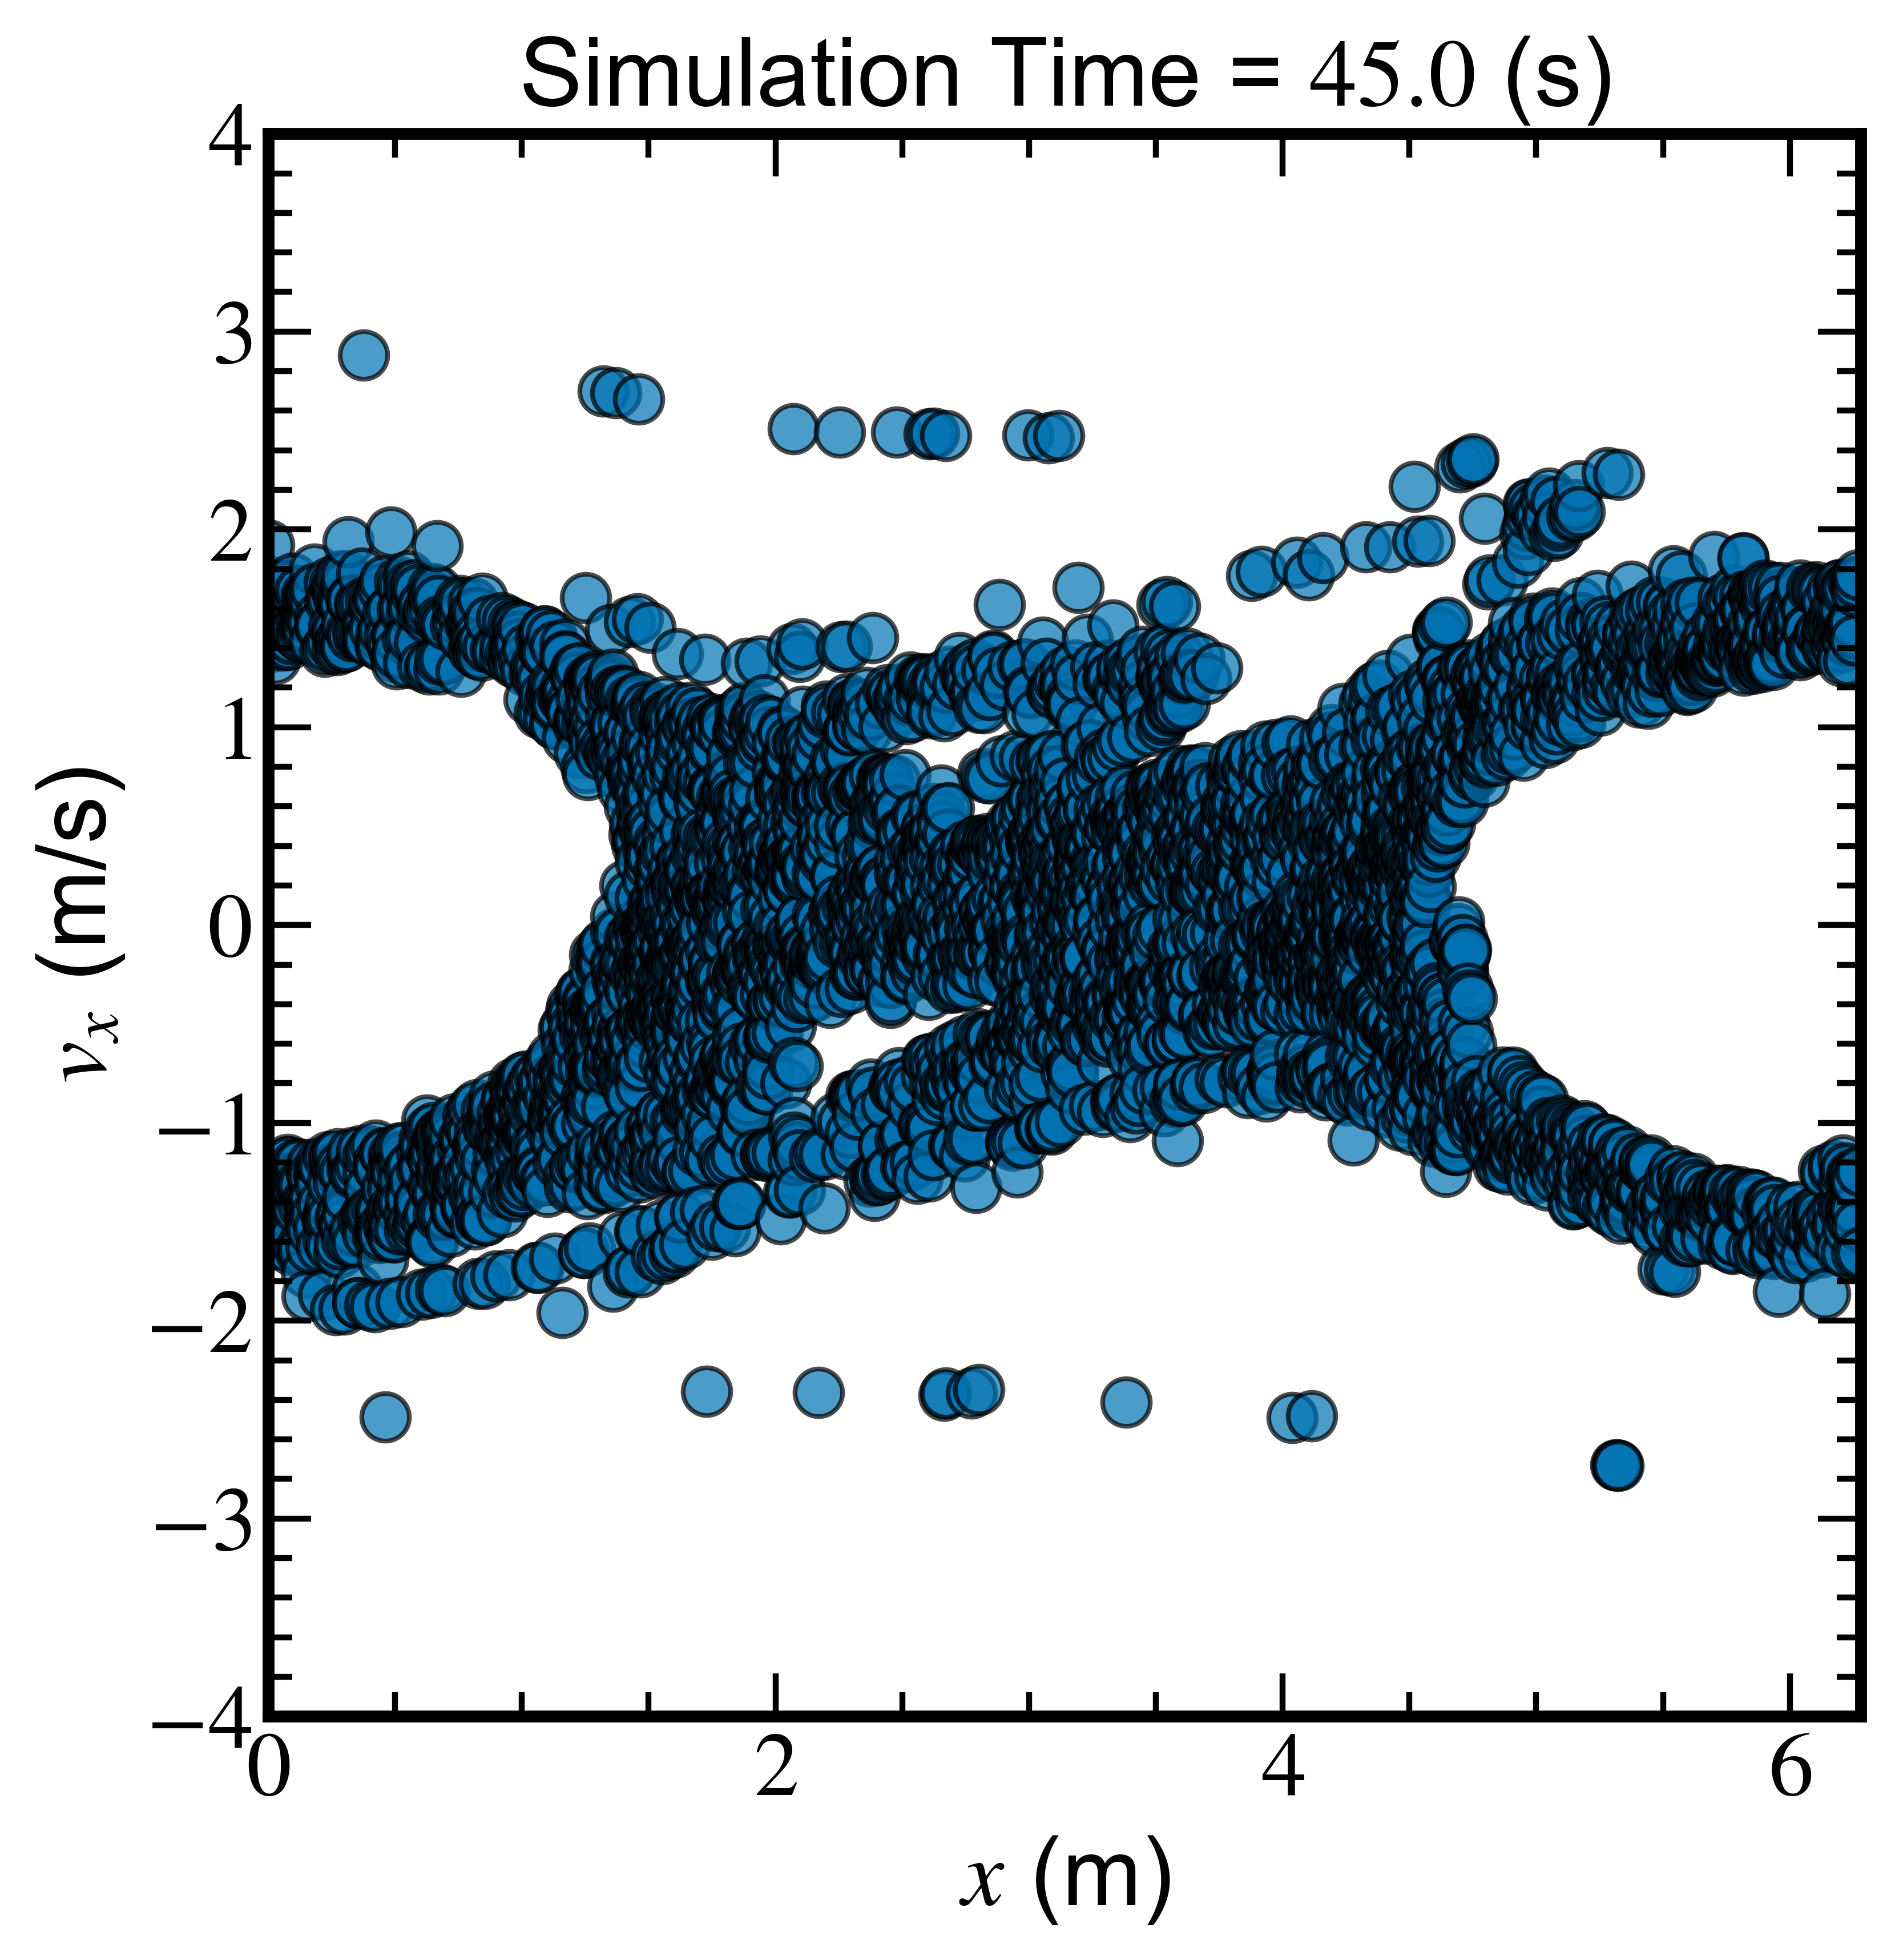
\includegraphics[width=0.5\textwidth]{figs/two_stream_frame_2.png}};
      \node[anchor=south west, inner sep=0] (image2) at (4,0) {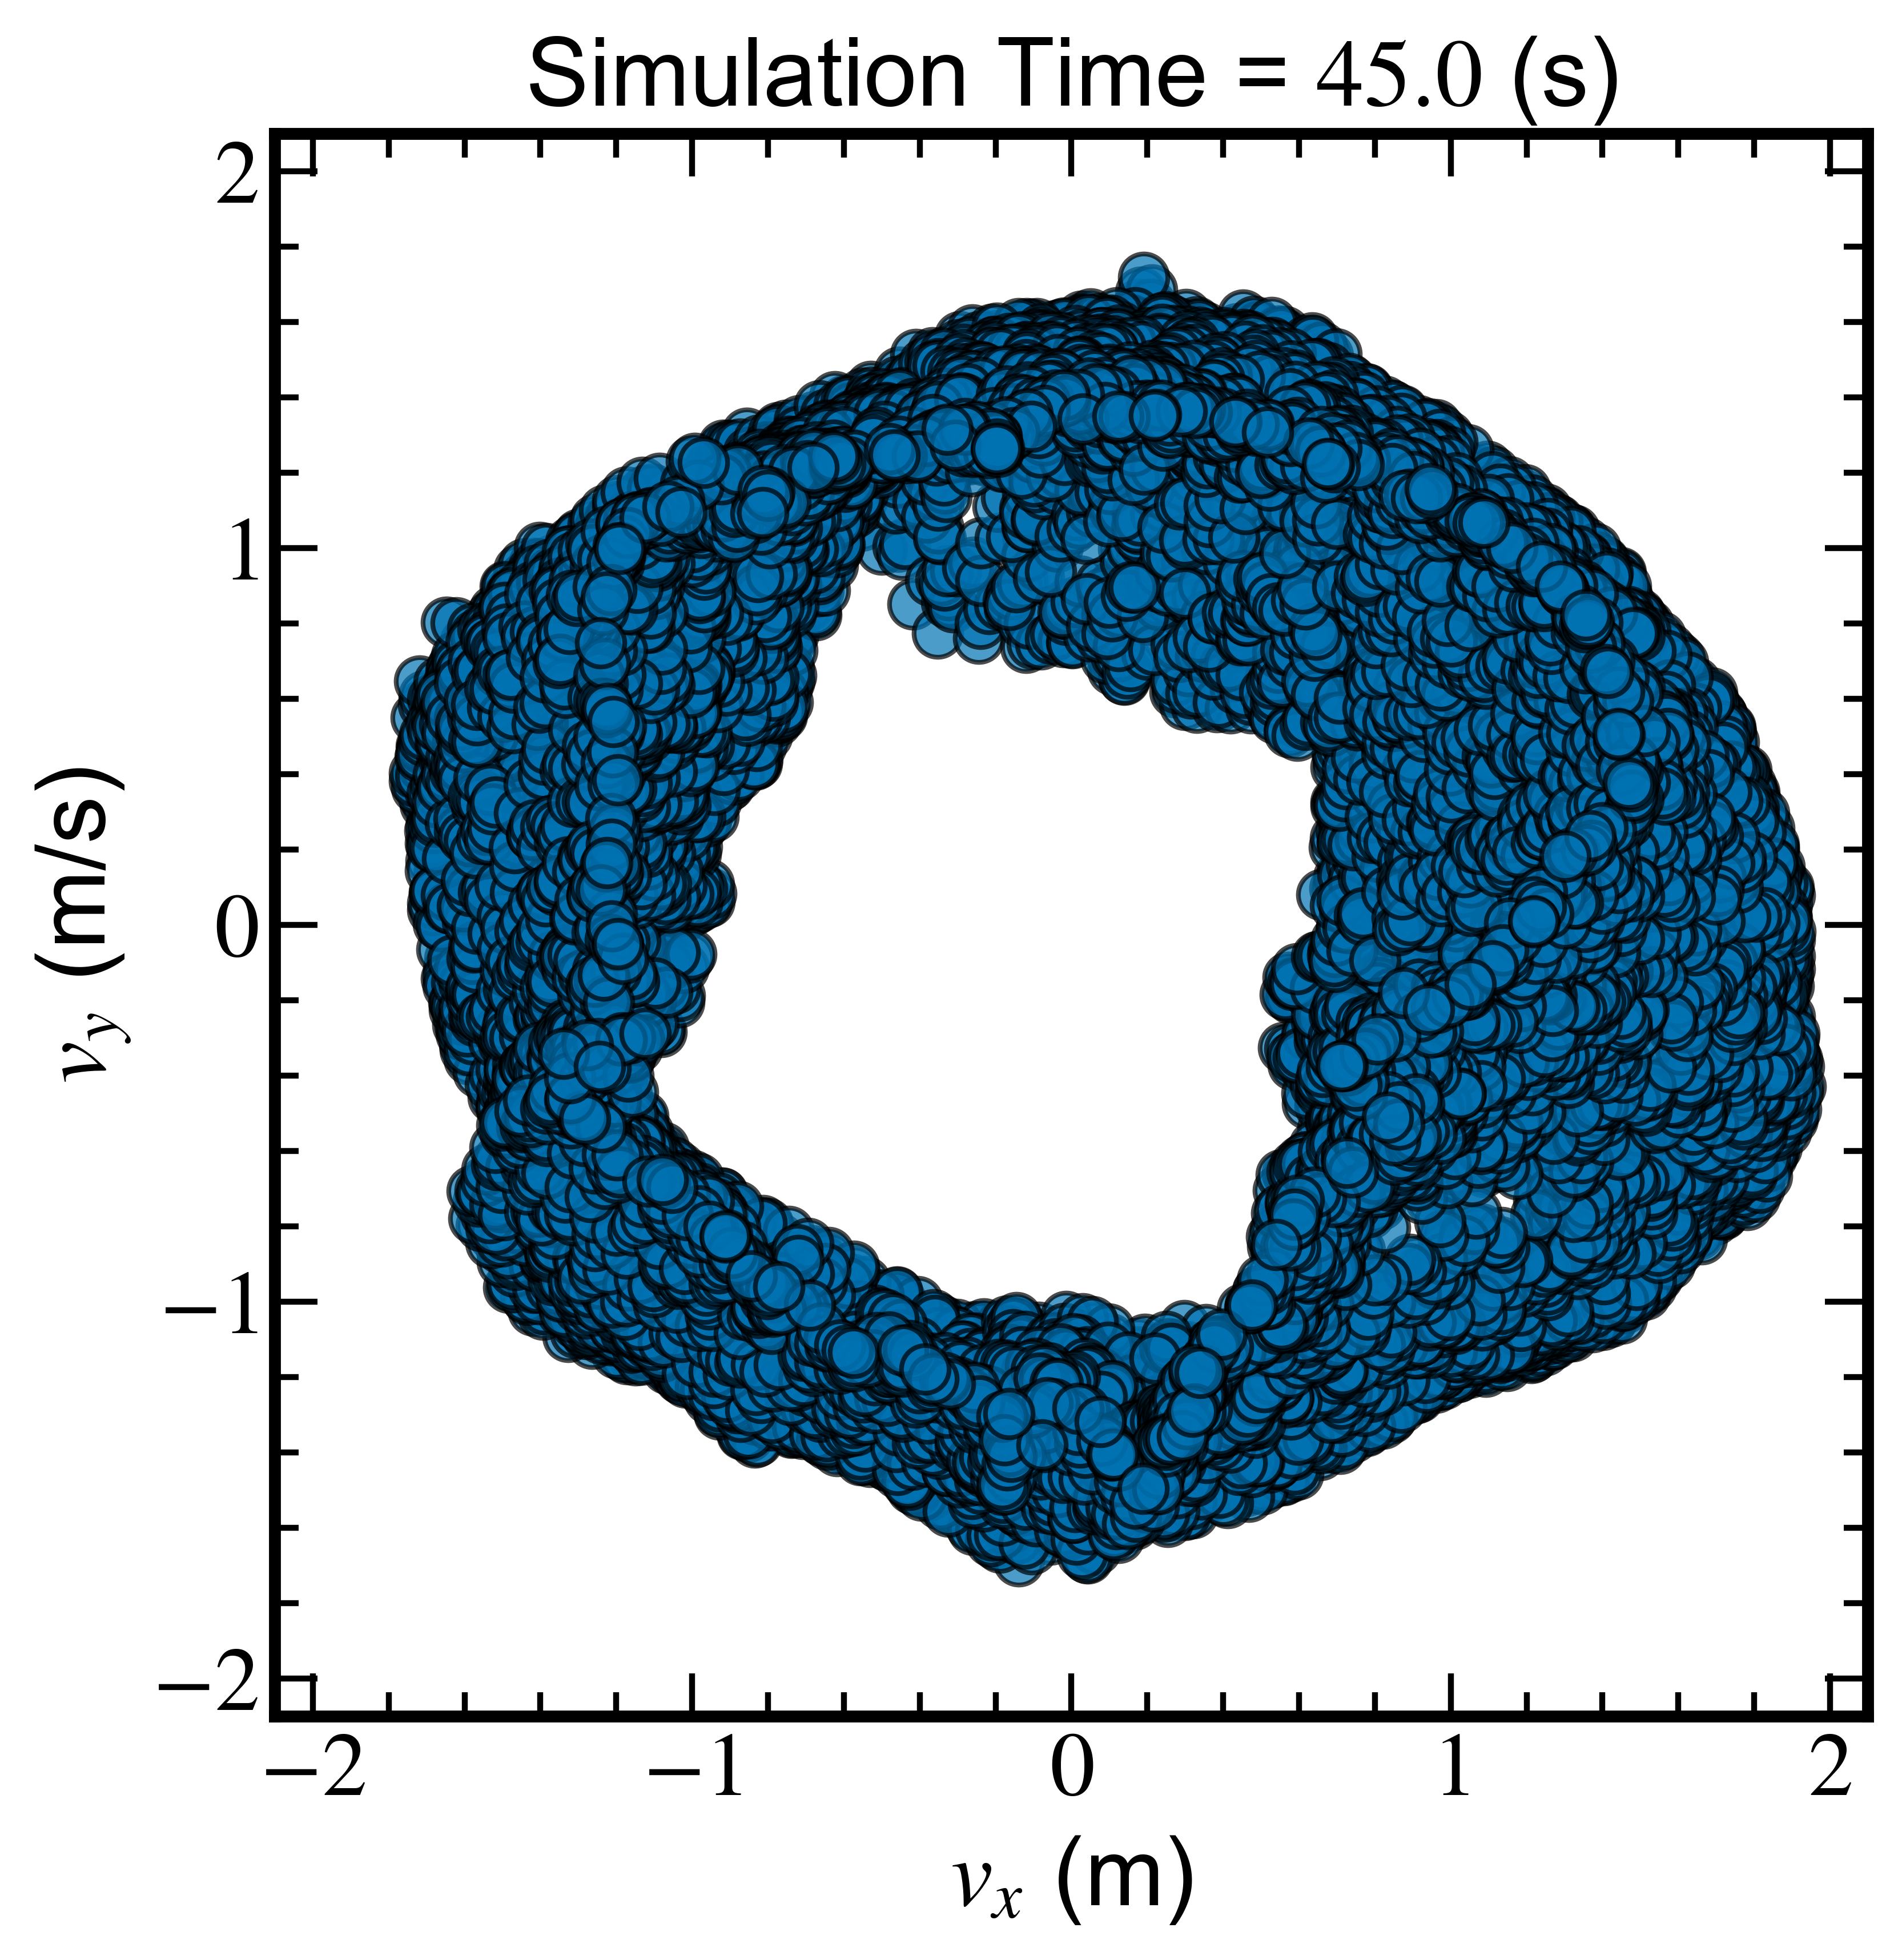
\includegraphics[width=0.5\textwidth]{figs/dgh_frame_2.png}};
  % Second image, overlapping top-right corner of image1
      \node[anchor=south west, inner sep=0] (image3) at (2, -2.75)
      {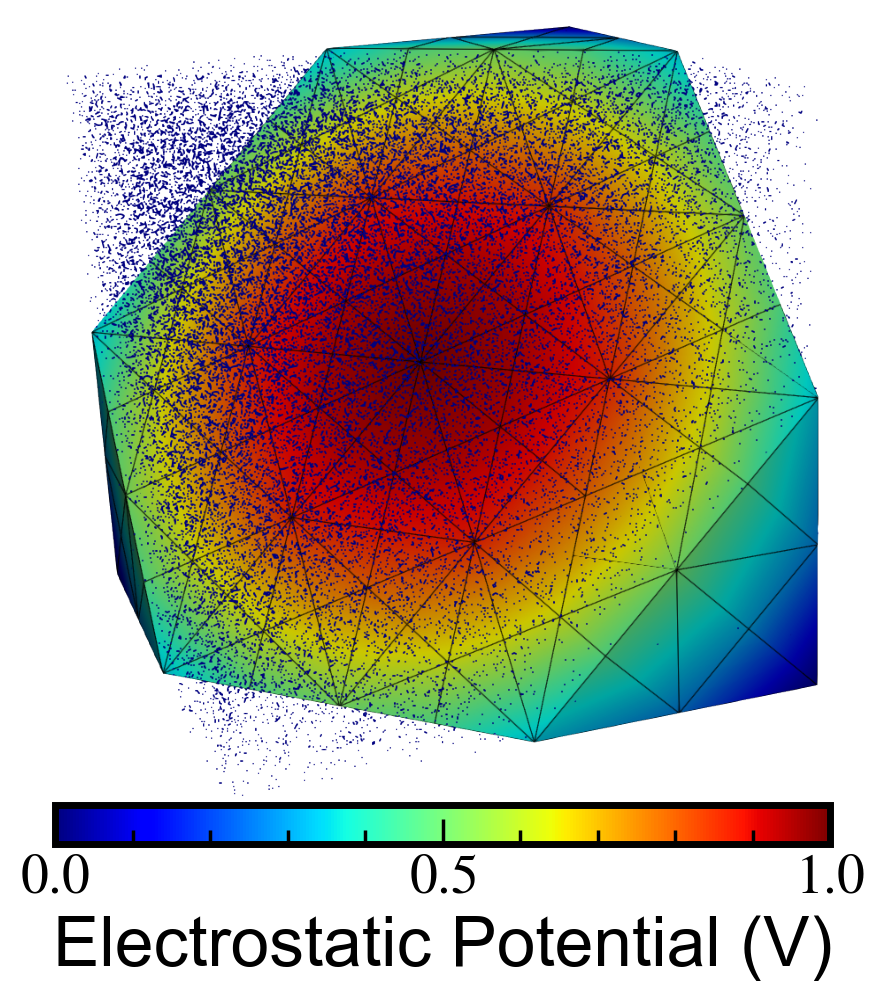
\includegraphics[width=0.5\textwidth]{figs/potential_visualization.png}};
    \end{tikzpicture}
    \end{figure}
  \end{columns}
  \vspace{-1cm}
\end{frame}
